
\documentclass{beamer}

%\usepackage[table]{xcolor}
\mode<presentation> {
  \usetheme{Boadilla}

%  \usetheme{Pittsburgh}
%\usefonttheme[2]{sans}
\renewcommand{\familydefault}{cmss}
%\usepackage{lmodern}
%\usepackage[T1]{fontenc}
%\usepackage{palatino}
%\usepackage{cmbright}

\useinnertheme{rectangles}
}

\setbeamercolor{normal text}{fg=black}
\setbeamercolor{structure}{fg= blue}
\definecolor{trial}{cmyk}{1,0,0, 0}
\definecolor{trial2}{cmyk}{0.00,0,1, 0}
\definecolor{darkgreen}{rgb}{0,.4, 0.1}
\usepackage{array}
\beamertemplatesolidbackgroundcolor{white}  \setbeamercolor{alerted
text}{fg=red}
\usepackage{tcolorbox}
\setbeamertemplate{caption}[numbered]\newcounter{mylastframe}


\usepackage{tikz}
\usetikzlibrary{arrows}
\usepackage{colortbl}

\renewcommand{\familydefault}{cmss}
%\usepackage[all]{xy}

\usepackage{tikz}
\usepackage{lipsum}

 \newenvironment{changemargin}[3]{%
 \begin{list}{}{%
 \setlength{\topsep}{0pt}%
 \setlength{\leftmargin}{#1}%
 \setlength{\rightmargin}{#2}%
 \setlength{\topmargin}{#3}%
 \setlength{\listparindent}{\parindent}%
 \setlength{\itemindent}{\parindent}%
 \setlength{\parsep}{\parskip}%
 }%
\item[]}{\end{list}}
\usetikzlibrary{arrows}

\usecolortheme{lily}

\newtheorem{com}{Comment}
\newtheorem{lem} {Lemma}
\newtheorem{prop}{Proposition}
\newtheorem{condition}{Condition}
\newtheorem{thm}{Theorem}
\newtheorem{defn}{Definition}
\newtheorem{cor}{Corollary}
\newtheorem{obs}{Observation}
 \numberwithin{equation}{section}
 

\setbeamertemplate{navigation symbols}{}


\title[PLSC 43401]{Mathematical Foundations of Political Methodology}

\author{Robert Gulotty}
\institute[Chicago]{University of Chicago}
\vspace{0.3in}


\begin{document}
\begin{frame}
\titlepage
\end{frame}


\begin{frame}{Review Topics}

\begin{itemize}
\item Probability and Mathematical Logic
\item Random Variables
\item Discrete PMF and CMF
\item Moments
\item Continuous Joint Distributions
\end{itemize}

\end{frame}





\begin{frame}{Probability Problems}

\begin{itemize}

\item Q. When do I use Bayes' Rule and when do I not? \pause
\item A. Bayes Rule is for when you have $P(B|A)$ but you need $P(A|B)$.  \pause
\item Example: I know what the chances of an infection given I have the disease, I see an infection and want to know if I have the disease.\pause
\item Q. When do I use the Law of Total Probability? \pause
\item A. Law of Total Probability is used when you want to aggregate the probability of an event across some partitioned space.\pause
\item Example: I know that Americans are either Republicans, Independents or Democrats, and I have information about each type of person's behavior, what should I expect?
\end{itemize}

\end{frame}

\begin{frame}{Boole's Inequality}

\begin{itemize}

\item $P(A\cup B) = P(A)+P(B)-P(A\cap B)$
\item $P(A\cup B) \leq P(A)+P(B)$
\end{itemize}

\end{frame}

\begin{frame}{Probability Rules: Unions and Intersections}

\begin{itemize}

\item $P(A\cup B) = P(A)+P(B)-P(A\cap B)$\pause
\item So if A and B are disjoint: $P(A\cup B) = P(A)+P(B)$.\pause
\item Example:
\item My dog, Maeby, will only bark at skateboards or salt spreaders.  We see skateboards when it is warm, salt spreaders when it is cold. \pause
\item We see skateboards with probability .1, \\We see salt spreaders with probability .2.\pause
\item The chance of barking is then $.1+.2=.3$
\end{itemize}

\end{frame}

\begin{frame}{Boole's Inequality}

\begin{itemize}

\item $P(A\cup B) = P(A)+P(B)-P(A\cap B)$
\item $P(A\cup B) \leq P(A)+P(B)$
\end{itemize}

\end{frame}




\begin{frame}{Probability Rules: Independence}

\begin{itemize}
\item $P(A|B)=\frac{P(A\cap B)}{P(B)}$\pause
\item If A and B are independent, $P(A|B)=\frac{P(A)P(B)}{P(B)}=P(A)$
\item If A is a subset of B, then $P(A|B)=\frac{P(A)}{P(B)}$\pause
\item Example:
\item Maeby only wears her boots when there is lots of salt.\pause
\item There is lots of salt only in occasions there is snow.\pause
\item $P(boots|snow)= \frac{P(boots)}{P(Snow)}$\
\end{itemize}

\end{frame}

\begin{frame}
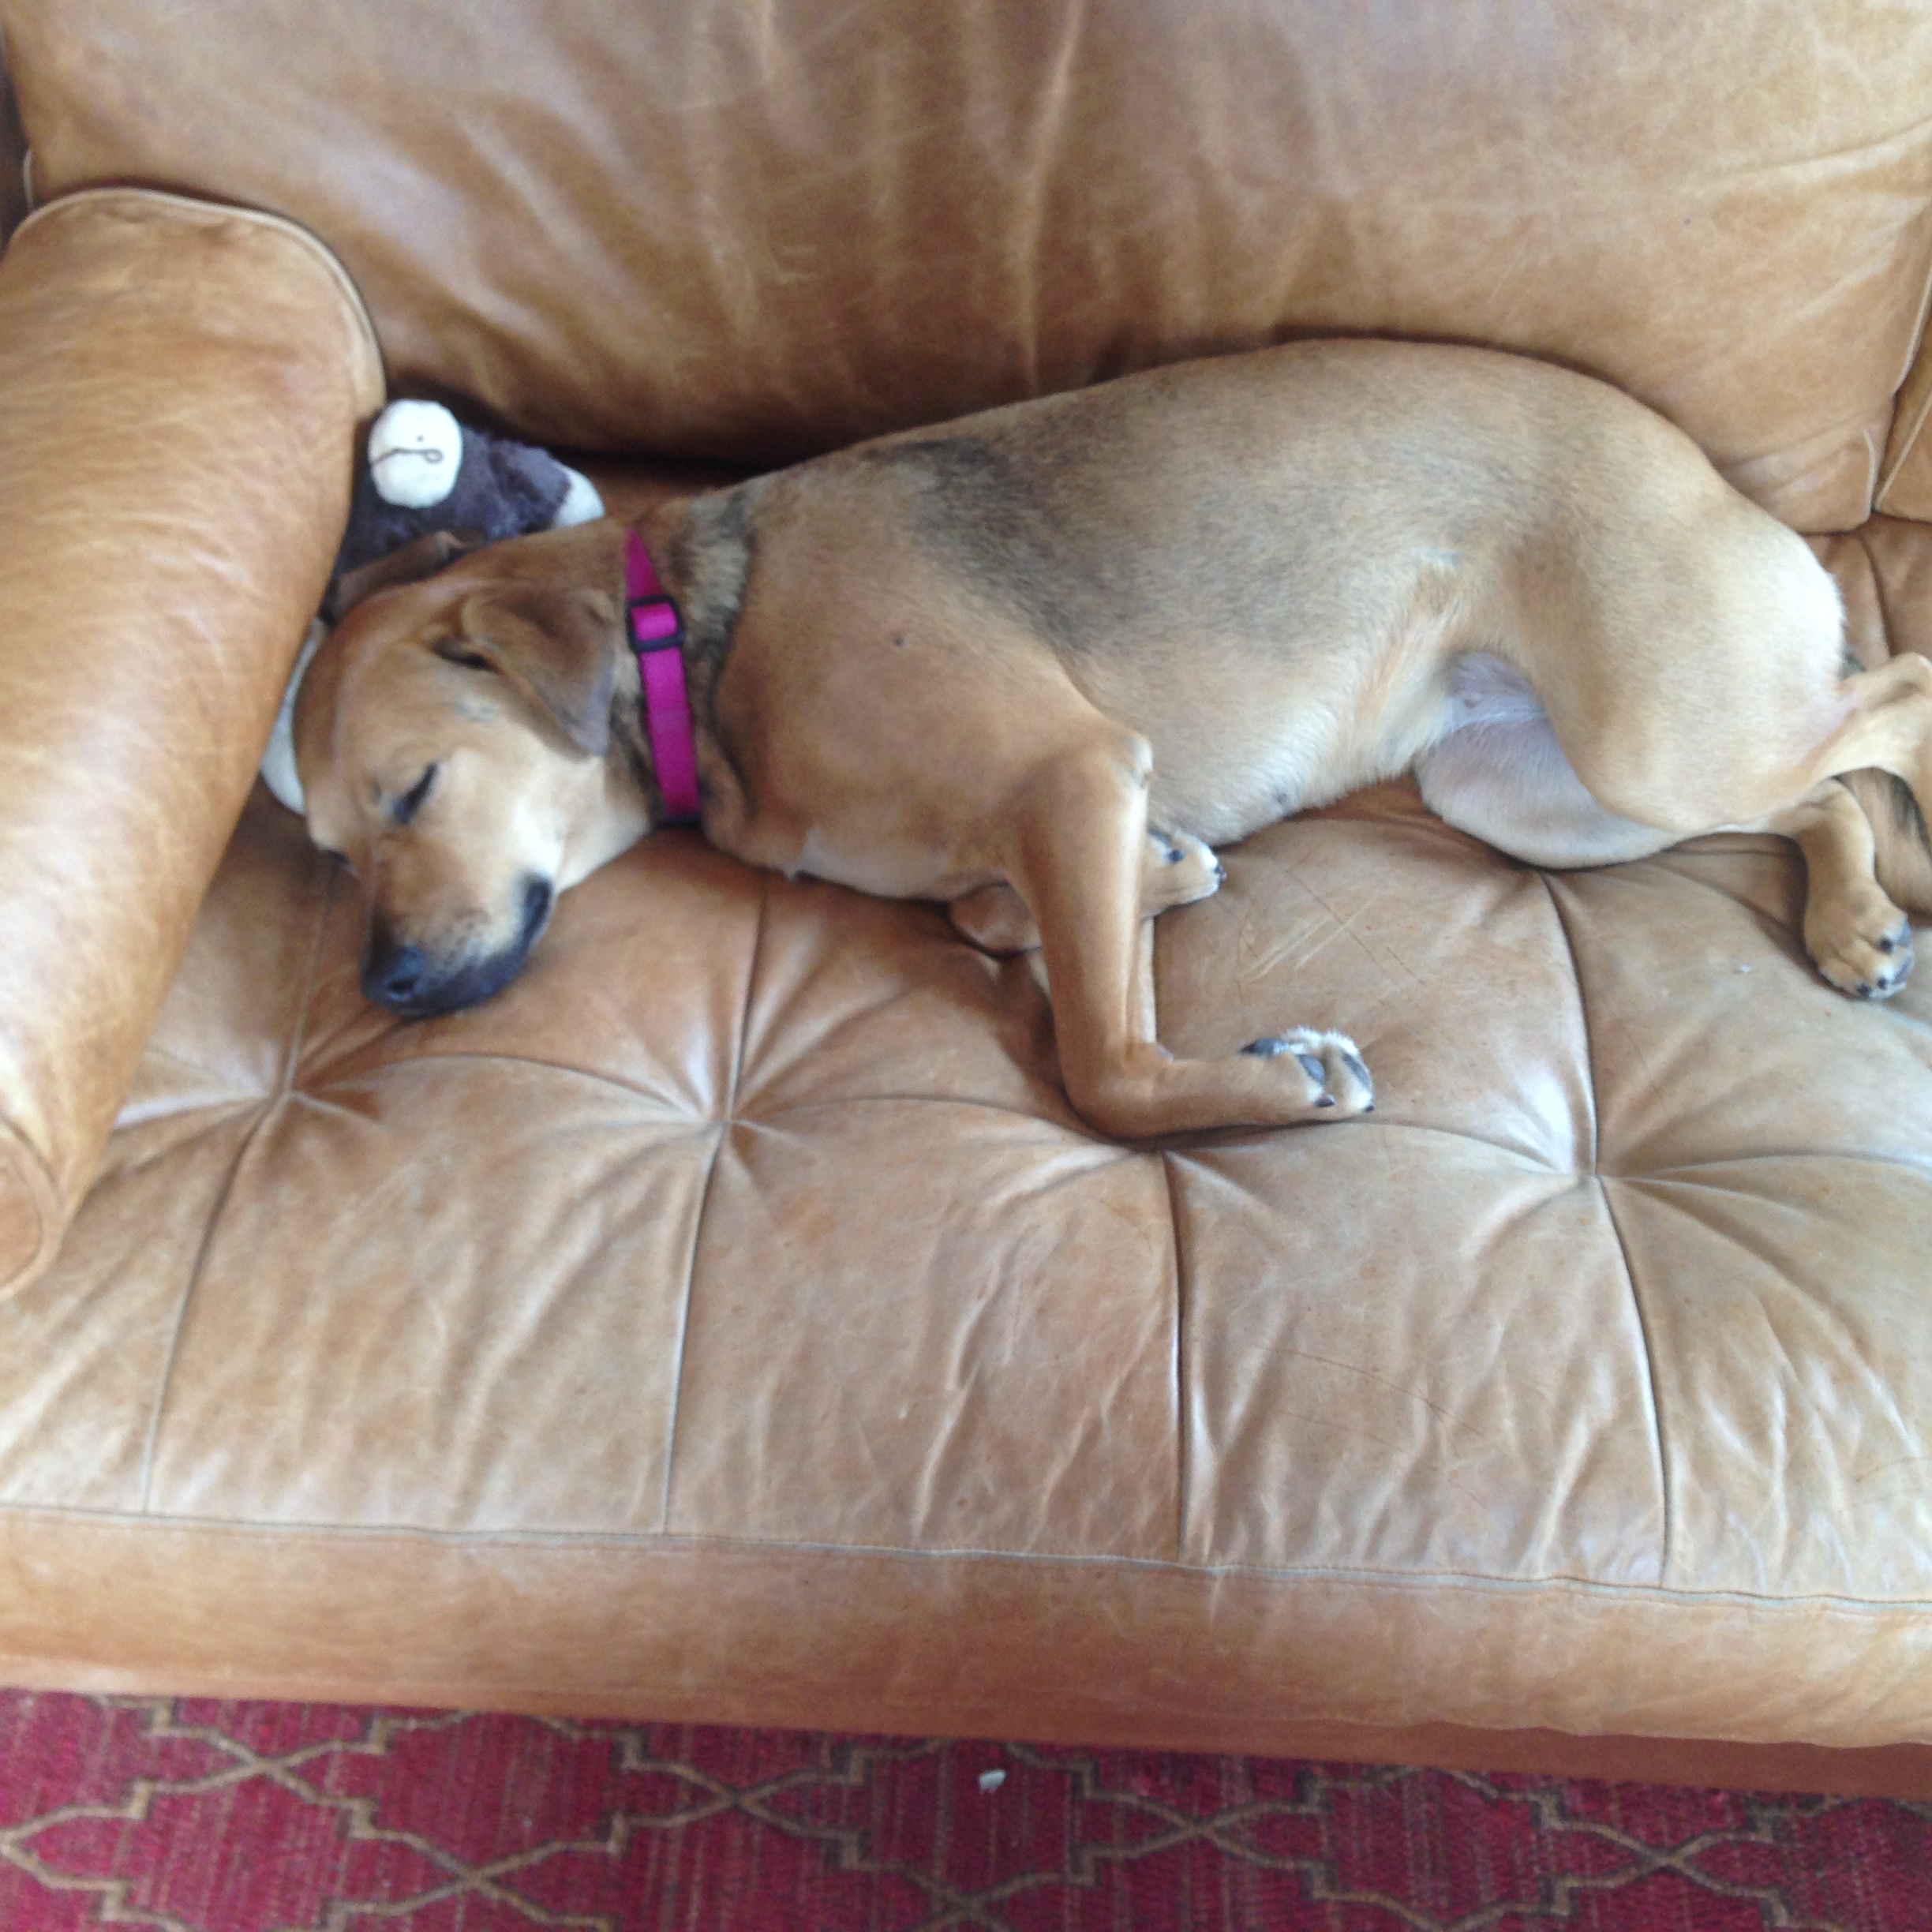
\includegraphics[width=4 in]{dog.jpg}
\end{frame}

\begin{frame}{Random Variables}

\begin{itemize}

\item A random variable is a function that assigns numbers to events.
\item A distribution tells us how likely those underlying events are. 
\item A histogram describes the probability of each discrete outcome.
\item A density plot describes the shape of continuous probability distributions.
\item Very important to distinguish discrete ($\sum$) random variables from continuous ($\int$) random variables.
\end{itemize}

\end{frame}

\begin{frame}{Binomial Example of PMF}

\begin{itemize}

\item Suppose that one out of every five witnesses will support the president.
\item We had four witnesses yesterday.
\item What is the expected number to support the president? 
\end{itemize}
\end{frame}


\begin{frame}{Binomial Example}
$$p(x)= {n \choose k}p^k (1-p)^{n-k}$$

If $n=4$ and $p=.2$ What is E(X)?

$$E(X)=\sum_{i\in \{0,\ 1,\ 2,\ 3,\ 4\}} x p(x)$$\pause
$$0 * {4 \choose 0}p^0 (1-p)^{4-0}+1 * {4 \choose 1}p^1 (1-p)^{4-1}+$$
$$2 * {4 \choose 2}p^2 (1-p)^{4-2}+3* {4 \choose 3}p^3 (1-p)^{4-3}+4 * {4 \choose 4}p^4 (1-p)^{4-4}=$$\pause
$$ 4 p (1-p)^{3}+12 p^2 (1-p)^{2}+12p^3 (1-p)+4 p^4 =$$\pause
$$ 4 *.2 (.8)^{3}+12 *.2^2 (.8)^{2}+12*.2^3 (.8)+4* .2^4 =0.8$$

\end{frame}



\begin{frame}{Moments}
\begin{itemize}
\item Archimedes noticed that levers apply torque equal to the product of the length of the lever (r) and the amount of effort (F). \pause
\item Now imagine you are spinning, the spread of your arms matters for how fast you will go and how resistant you are to change.\pause
\item The center of gravity of an object (first moment) vs the swing radius (second moment).\pause
\begin{itemize}
\item $E(X)=\int x f(x)dx$ is called the first moment.
\item $E(X^2)=\int x^2 f(x)dx$ is the second moment.
\item $E(X^3)=\int x^3 f(x)dx$ is the third moment (skewness)
\item $E(X^4)=\int x^4 f(x)dx)$ is the fourth moment (kurtosis)
\end{itemize}
\end{itemize}
\end{frame}



\begin{frame}{Cumulative Poisson Distribution}

\begin{itemize}
\item Suppose we impeach a president four times in 243 years.  4/243 \pause
\item What is the chance of impeaching more than two more in our lifetimes (80 years)? \pause
\item $\lambda= 4/243*80 =1.3$ \pause
\item The CDF of the Poisson distribution is $F(X\leq k)=e^{-\lambda}\sum_{i=0}^k \frac{\lambda^i}{i!}$ \pause
\item The probability of more than 2 in 80 years is $1-F(X\leq 2)$ \pause
\end{itemize}

$$=1-e^{-\lambda}\sum_0^k \frac{\lambda^i}{i!}=1-e^{-1.3}[ 1+ 1.3+ \frac{1.3^2}{2}]$$
$$=1-.857=.143$$
\end{frame}


\begin{frame}{Conditional Expectations with One Variable}
$$f_{X|{X\in A}}(x)=\frac{f_X(x)}{P(X\in A)}$$
$$E(X|X\in A)=\int x f_{X|{X\in A}}(x)$$

So if $f_x$ is the Uniform (-1, 1)
\begin{itemize}
\item What is $f_{X|X>0}(x)$?
\item What is $E(X|X>0)$?
\end{itemize}
\end{frame}




\begin{frame}{Example of Joint Density of X and Y}

$$f(x,\ y)= e^{-x/y}\cdot \frac{e^{-y}}{y} \quad \text{if } x,\ y >0$$
\begin{itemize}
\item Find marginal distribution of Y.
\item Check whether f(x,\ y) is a valid pdf.
\item Find $E(Y)$
\item Find conditional distribution of X given Y=y.
\end{itemize}

\end{frame}
\begin{frame}{Marginal distribution of Y}

$$f(x,\ y)= e^{-x/y}\cdot \frac{e^{-y}}{y} \quad \text{if } x,\ y >0$$

\begin{itemize}
\item Procedure: Take integral of joint pdf with respect to X.
\end{itemize}
$$f(y)=\int_{-\infty}^\infty f(x,\ y) dx$$\pause
$$f(y)= \int_{0}^\infty e^{-x/y}\cdot \frac{e^{-y}}{y} dx$$\pause
$$f(y)= \frac{e^{-y}}{y}\int_{0}^\infty e^{-x/y}dx$$\pause
$$f(y)= \frac{e^{-y}}{y}  [-y e^{-x/y}|_\infty - -y e^{-x/y}|_0]$$\pause
$$f(y)= \frac{e^{-y}}{y}  [0 + y] =e^{-y}$$
\end{frame}


\begin{frame}{Check if f(x,\ y) is a pdf.}

$$f(x,\ y)= e^{-x/y}\cdot \frac{e^{-y}}{y} \quad \text{if } x,\ y >0$$

\begin{itemize}
\item Procedure: Take integral w.r.t. X then Y and see if it is equal to 1.
\end{itemize}
$$\int_{-\infty}^\infty \int_{-\infty}^\infty f(x,\ y) dxdy$$\pause
$$=\int_{0}^\infty[ \int_{0}^\infty e^{-x/y}\cdot \frac{e^{-y}}{y} dx]dy$$\pause
$$= \int_{0}^\infty[ \frac{e^{-y}}{y}\int_{0}^\infty e^{-x/y}dx]dy$$\pause
$$= \int_{0}^\infty[\frac{e^{-y}}{y}  [-y e^{-x/y}|_\infty - -y e^{-x/y}|_0]dy$$\pause
$$=\int_{0}^\infty[ \frac{e^{-y}}{y}  [0 + y]]dy =\int_{0}^\infty e^{-y}dy=1$$
\end{frame}



\begin{frame}{Find $E(Y)$}
\begin{itemize}
\item Procedure: take integral of values of y times density of y.
\end{itemize}
$$E(Y)=\int_{-\infty}^\infty y\cdot f(y) dy$$\pause
$$=\int_{0}^\infty y\cdot e^{-y} dy$$\pause
\emph{Integrate by parts}:\\ $\int u dv = uv-\int v du$, $dv= e^{-y}$, $v=-e^{-y}$, $u=y$, $du=1$\pause
$$=[-ye^{-y}]_0^\infty - \int_0^\infty -e^{-y}dy$$\pause
$$=0-0 +1=1$$\pause
Alternatively, one could recognize that $Y\sim Exp(1)$
\end{frame}


\begin{frame}{Find conditional distribution of X given Y=y.}
\begin{itemize}
\item Procedure: use definition of conditional $f(x|y)=\frac{f(x,\ y)}{f(y)}$
\end{itemize}
 $$f(x|y)=\frac{e^{-x/y}\cdot \frac{e^{-y}}{y}}{e^{-y}}$$\pause
 $$f(x|y)=\frac{1}{y}\cdot e^{-x/y}$$

\end{frame}

\begin{frame}
\includegraphics[width=4 in]{dog2.jpg}
\end{frame}




\end{document}